% using Elseveir template per https://www.elsevier.com/authors/author-schemas/latex-instructions
\documentclass[review]{elsarticle}
\usepackage{lineno,hyperref}
\modulolinenumbers[5]
\bibliographystyle{elsarticle-num}

\usepackage{booktabs}
\usepackage{graphicx}
\graphicspath{{../alt-ed-survey/figures-and-tables}}
\usepackage{hyperref}
\usepackage{threeparttable}  
\usepackage{tikz}
\usetikzlibrary{calc,matrix}

\begin{document}
\begin{frontmatter}

    \title{
        COVID-19 and Alternative Postsecondary Learning
        % \tnoteref{titlenotes}
    }
    % \tnotetext[titlenotes]{
    %     Go to \url{https://github.com/Vandivier/research-dissertation-case-for-alt-ed/tree/master/papers/alt-ed-survey}
    %     for additional materials including the online appendix,
    %     survey data, and data analysis source code.
    % }

    \author[mymainaddress]{John Vandivier}
    \address[mymainaddress]{4400 University Dr, Fairfax, VA 22030}
    \ead{jvandivi@masonlive.gmu.edu}
    % \fntext[authorlinefootnote]{
    %     Vandivier: George Mason University,
    %     4400 University Dr, Fairfax, VA 22030,
    %     jvandivi@masonlive.gmu.edu.
    % }

    \begin{abstract}
        The coronavirus pandemic has induced an increase in remote activity.
        Prior research shows that a variety of K-12 educational practices, public preferences, policies, and outcomes
        have changed as a result of the pandemic.
        This paper extends the literature on the impact of coronavirus on education
        to solve for the lack of analysis on professional certifications
        and other unaccredited postsecondary credentials.
        This paper investigates the results of an original online questionnaire ($n = 350$)
        to understand the effects of COVID-19
        on support for alternative postsecondary learning.
        Respondents are U.S. citizens over the age of 18.
        Cross-sectional analysis using ordinary least squares (OLS)
        and Iteratively Reweighted Least Squares (IRLS)
        indicates that individual perception of a large negative impact from coronavirus
        is significantly correlated with
        higher favorability to alternative credentials.
        Analysis indicates that important control factors include industry, ethnicity, and state of residence.
        Age, gender, income, and level of education are insignificant.
    \end{abstract}

    \begin{keyword}
        education economics, alternative education, coronavirus             %%% not grammatical
        \MSC[2010] I12, I21, I23 % Also could use I24, I25, I28             %%% not grammatical
    \end{keyword}

\end{frontmatter}

\pagebreak
\linenumbers

\section{Introduction}

This study is concerned with alternative postsecondary credentials.
This category includes professional certifications, coding bootcamps, work portfolios,
and other proof of education other than traditional credentials.
In this study, traditional credentials mainly refer to the accredited college degree.
Remote learning was an alternative approach to education from inception, and it continues to be deeply involved in alternative learning.
This study hypothesizes that the impact of coronavirus is positive on favorability to alternative credentials.
Results favor the hypothesis, with evidence that exposure to remote learning is a critical mechanism.

There are three theoretical reasons to suppose that a pandemic would make alternative postsecondary credentials more attractive.
The first is that the pandemic response has resulted in exposure to remote activity,
and exposure effects are often positive on favorability.
Second, alternative learning providers face different incentives compared to traditional providers.
Differing incentives may provide an adaptive advantage in the face of rapid social change.
A recent paper on organizational agility in higher education points to regulatory challenges
and deep, centralized, hierarchical organizational structure as notable disadvantages\cite{menon2020factors}.

The third theory is that a pandemic is a time when normal strangeness increases across society.
When the normal level of strangeness increases, things that were already finitely strange become relatively less strange.
Alternative credentials are strange in some sense by construction,
but the relative stigma associated with these credentials might decrease in a time like that of the present pandemic,
where all sorts of previously strange behaviors have become a new normal.
% Suppose that a strange thing becomes less strange when it is logically explained.
% In this case, remote activity plays a logical role as a social distancing solution, 
% and benefits to favorability from remote activity are not clearly reduced to mere exposure effects.
% Moreover, any stigma associated with a person selecting cheap education becomes less of an issue
% when the logic that a pandemic causes general financial difficulty is accounted for.
% This becomes more plausible when the connection of alternative credentials to remote activity is highlighted.
% At a time when personal contact is costly,
% remote learning becomes a better bargain,
% and the social benefits of traditional education are simultaneously diminished.

% This would theoretically reduce any relative stigma which the alternatively educated invididual might face.
% The stigma is reduced by two mechanisms.
% First, society changes many norms during a pandemic, so the general strength of social norms is reduced.
% In this way, the general preference for traditional over alternative education is reduced.
% Secondly, consuming alternative education is specifically reasonable as a pandemic adaptation.
% During a pandemic, many of the attractions of university life are unusable,
% remote learning provides protection against becoming ill,
% and pinching pennies is more understandable than it is during times of flourishing.
% When an individual has such good reasons for pursuing alternative education, it becomes unreasonable to impose a stigma at hiring decision time.
% TODO: the above is related to mitigation tactics for disabled people during interview; stigma management...idk the exact keywords look it up

% The third reason that a pandemic could make a massive shift to alternative learning more reasonable
% is simply that massive shifts are less spectacular in a time of pandemic.
% Society has already changed many norms in the face of the pandemic.
% Some of these norm changes are directly linked while others are indirect.
% Social distancing, wearing masks, fewer shaken hands, and so on, are some direct measure.
% The lack of fresh bread at my local coffee shop is an indirect change resulting from supply chain cost impact of the pandemic.
% Both are understandable changes.
% In this pandemic context an empathetic employer would look at an alternatively educated individual as making a reasonable adaptation,
% whereas previously they might face some stigma for making a strange choice.
% In a time where many norms are being disrupted, there may be an external effect which weakens norms in general,
% and therefore the general preference of traditional to alternative education would.

While exposure to some stigma generally increases favorability, there are several special cases where it declines instead.
Coronavirus-induced exposure could be such a case of negative exposure for a few reasons.
Direct exposure to disease is generally harmful, unwanted, and forced.
Disease-induced activities are not strictly involuntary,
but they might be perceived disfavorably by association.
The mere exposure effect\cite{robinson2005novel} and familiarity bias\cite{cao2011fear}
are generally positive on favorability to some stimulus,
but these exposures are often voluntary.
Unwanted exposure that involves harm tends to reduce favorability.
Backfire, boomerang, and blowback effects are examples of a negative response to exposure
\cite{swire2020searching, byrne2009boomerang, campagna2016strategic}.
One study relates closely to the COVID-19 pandemic in finding a backfire effect in efforts to market flu vaccine usage
\cite{nyhan2015does}.
Interestingly, repeated negative exposure can lead to positive favorability,
as documented in work on Stockholm syndrome\cite{julich2005stockholm}.
% Pain toleration can also lead to reduction in negative stimulus response

The exposure effect of coronavirus and related social changes might reflect a combination of the above effects.
As a result, the direction of effect is not apparent without empirical study.
Individual favorability to alternative credentials is also like to vary for various personal reasons unrelated to the pandemic.
This paper uses multiple regression to hold these sources of variation constant.

There are already several papers examining the impact of coronavirus on the education system.
These papers focus on education from kindergarten through high school,
but they inspire the hypothesis of a similar situation in higher education.
One paper in the Journal of School Choice examined the educational experiences of families under COVID-19\cite{carpenter2020we}.
The study found that 57 percent of parents found remote learning worked better than they expected.

% TODO: cite four papers and show how they relate
% TODO: why do we care about these credentials? 1 higher quality, 2 lower price, 3 faster, 4 align to workforce needs, 5 solve for equity/equality
% TODO: alt creds vs alt ed? signalling theory says credentials communicate value;
%       from a modeling perspective they make alt ed concrete by demarking achievement for factor attribution
% TODO: BLS data: "postsecondary nondegree award"
% TODO: other orgs? saylor academy, lumina foundation, credly/acclaim, ACE gov body, (OER) open ed resources much online, 'skill gap'
% TODO: why remote learning matters? even traditional is moving that way
% TODO: why would remote learning correlate with alternative credentials? a few reasons:
%   1. online learning is itself an early form of alternative education. It is not a traditional pedagogy.
%   2. online learning has a historical connection with edtech;
%      edtech is generally the perview of alternative providers precisely because change and innovation are slow at the traditional institution
%   as an aside, the highlights again the special role of the information technology industry; edtech is a subsection of IT.

\section{Description of Data and Methodology}

This paper leverages an original set of online questionnaire responses ($n = 350$).
Responses are cross-sectional data obtained in early February of 2021,
about one year after a public health emergency due to the coronavirus outbreak was declared in the United States\cite{staff_2021}.
Respondents are United States citizens at or over the age of eighteen.
Qualified respondents participated in the survey through the Amazon Mechanical Turk platform.

This study uses multiple regression of linear and curvilinear factors to generate results
\footnote{
    While the data for this analysis is not public, the analytical code is open-source.
    See \url{https://github.com/Vandivier/research-dissertation-case-for-alt-ed/tree/master/papers/alt-ed-covid-2/data}
}.
Each model in this study follows an ordinary linear model or a robust linear model (RLM) specification.
Ordinary linear models compute factor coefficients using ordinary least squares (OLS),
and robust linear models use iteratively reweighted least squares (IRLS).
Factor coefficients across these models are comparable,
but RLM does not generate a useful R-squared statistic
for model-level comparison.
Robust linear models are useful to improve estimation when outliers exist\cite{sievers2004rank}
and 11 outliers exist in the sample.

Appendix A contains the exact wording and response options for each question.
Appendix A also contains the wording for a priming message presented at the start of the survey.
The priming message lays out the definition of alternative credentials for the purposes of the study.
The message also provides several concrete examples of alternative credentials,
including ``a Certified Project Manager certification,
a portfolio of work, a Khan Academy profile, or a Nanodegree from Udacity.''

The questionnaire is composed of fourteen questions.
Favorability is the dependent variable of interest.
Coronavirus impact is the independent variable of interest.
There are also ten control factors and two questions on causality.

% TODO: cite a couple papers
Eight of the ten control factors are common controls in the literature.
These eight controls are categorical measures for
for age, gender, ethnicity, income,
level of education, employment status, the industry of occupation, and state of residence.

The two remaining controls are unique to this study.
Expected conventionality is the first unique control.
Expected conventionality is the term used to describe the response to question three in the appendix.
Expected conventionality explains the effect on favorability that is
attributable to the future social acceptability of alternative credentials.
Correcting for social acceptability allows the remaining effects to be interpreted more accurately as an individual preference.

% TODO: maybe talk about a couple papers that say mode of instruction is related to favorability
The second unique control is support for online education.
Online education is the response to question four in the appendix.
This control allows an analyst to hold constant the mode of instruction when interpreting favorability to alternative credentials.
% Mode of instruction is a bit of a red herring which is not what this study is centrally concerned with.
% Favorability to online education creates noise in the signal of favorability to alternative credentials,
% and this factor seperates that effect.
% The reason isolating this noise is important is because there are two assumptions in the mind of the respondent population.
% The first assumption is that traditional education involves in-person learning.
% The second assumption is that alternative education typically involves remote learning.
% Neither of these associations are held as true in the current analysis, so the introduction of this control allows
% Alternative education often employs remote learning, but this is not always the case.
% A respondent may still tend to associate the concepts and impute a halo effect from one to the other.
% This control allows an analyst to seperate favorability from alternative credentials

The primary interest of this study is to identify the effect of coronavirus on favorability.
If the effect of coronavirus is significant, a description of the origin of that effect improves the value of the results.
The two unique controls and the two questions about causality support investigation into exposure to remote activity as an explanation.
% Specifically, one hypothesized mechanism is that coronavirus stimulates remote activity,
% then exposure to remote activity improves favorability to all remote activities,
% then alternative credentials improve in favorability through a normative association with remote learning.

The variables of interest,
causality questions,
and the two unique controls obtain Likert-type responses.
The impact of coronavirus and the causality questions use a 4-point scale.
Favorability and the unique controls use a 10-point scale.
Continuous treatment of items on the 10-point scale permits curvilinear analysis,
allowing investigation of marginal effects
\footnote{
    It is an accepted practice to treat Likert-type responses as either categorical or continuous for regression analysis.
    Jaccard and Wan provide support for continuous analysis of Likert-type data.
    They note that severe departures from the assumptions on cardinality ``do not seem to affect Type I and Type II errors dramatically,''
    particularly when the Likert scale is five or more points\cite{jaccard1996lisrel}.
    This paper treats responses on a 10-point scale as continuous.
    This paper treats responses on a 4-point scale as categorical.
}.

\section{Results}

The median favorability response was eight out of ten.
Figure \ref{fig:one} visualizes the distribution of responses.
Of 350 responses, 11 responses indicate a favorability of less than four out of ten.
Regression analysis indicates a significant and positive coronavirus impact effect.
Analysis with and without outliers does not show a meaningful difference in the effect.
% The effect of the coronavirus impact on favorability
% is not held with confidence over the outlier range.

\begin{figure}[h!]
    \centering
    \caption{Distribution of Favorability to Alternative Credentials}
    \begin{tikzpicture}[element/.style={minimum width=1.75cm, minimum height=0.85cm}]
        \node (n1) {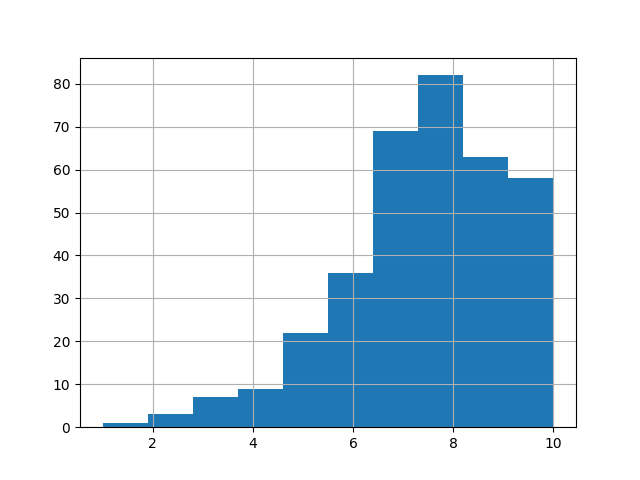
\includegraphics[width=0.7\textwidth]{./figures-and-tables/figure-1.png}};
    \end{tikzpicture}
    \label{fig:one}
\end{figure}

The average response was 7.65 on a 10-point scale.
Excluding outliers, over 96 percent of responses fall into the normal range.
The average response in the normal range was about 7.81.
Table \ref{tab:desc_stats} summarizes statistics about favorability and the direct measure of coronavirus impact.
The table also includes summary results for the two causality questions.

% Table \ref{tab:desc_stats} describes summary statistics for the total sample and also distinctly describes three subsamples.
Table \ref{tab:desc_stats} reports statistics across the total population and also for three subpopulations.
The subpopulations include the normal range, the outlier population, and the Tens.
Because factors in Table \ref{tab:desc_stats} dummy variables,
with an exception for favorability,
the mean values for each variable can be interpreted as the proportion of the population
that affirms the response.

The Tens are those individuals that responded with a favorability of 10 to alternative credentials.
The Tens are not an outlier group, but inspection of this group assists in understanding the response distribution.
The Tens report a large perceived impact at a disproportionately high rate.
In contrast, no member of the negative outlier group also reports a large perceived impact of coronavirus.
% Group differences like this demonstrate that general results for the whole American population are to be taken lightly,
% and 
% The difference in perceived impact by group is important when conclusions about the American population are drawn from the discussion on coronavirus impact.

This data is consistent with external reporting that COVID-19 impacts most Americans\cite{demographic2020},
but it adds the wrinkle that most Americans consider the impact to be minor.
Perceived COVID-19 impact is another case where outliers and Tens importantly differ from the average.
The Tens report higher coronavirus impact while the outliers cluster around a medium impact response.

\begin{table}
    \caption{Summary Statistics for Factors of Interest}
    \resizebox{\columnwidth}{!}{
        {
\def\sym#1{\ifmmode^{#1}\else\(^{#1}\)\fi}
\begin{tabular}{llcc}
    \toprule
                              &                                   & \textbf{Average Hirability} & \textbf{Average Prestige} \\
    \midrule
    \textbf{Actual Schools}   &                                   &                             & 6.50                      \\
                              & \textbf{Accredited}               &                             & 7.05                      \\
                              & \textbf{Unaccredited}             &                             & 6.07                      \\
                              & \textbf{Difference}               &                             & 0.98                      \\
    \cmidrule{2-4}
                              & \textbf{Stipulated High Prestige} &                             & 6.72                      \\
                              & \textbf{Stipulated Low Prestige}  &                             & 6.23                      \\
                              & \textbf{Difference}               &                             & 0.49                      \\
    \cmidrule{2-4}
    \textbf{Vignette Schools} &                                   & 6.49                        & 6.21                      \\
                              & \textbf{Accredited}               & 6.97                        & 6.49                      \\
                              & \textbf{Unaccredited}             & 6.02                        & 5.93                      \\
                              & \textbf{Difference}               & 0.95                        & 0.56                      \\
    \cmidrule{2-4}
                              & \textbf{Stipulated High Prestige} & 7.59                        & 7.69                      \\
                              & \textbf{Stipulated Low Prestige}  & 5.63                        & 4.94                      \\
                              & \textbf{Difference}               & 1.96                        & 2.75                      \\
    %   \midrule
    % \textbf{Pooled}           &                                   &                             & 6.37                      \\
    %                           & \textbf{Accredited}               &                             & 6.77                      \\
    %                           & \textbf{Unaccredited}             &                             & 6.01                      \\
    %                           & \textbf{Difference}               &                             & 0.76                      \\
    %                           & \textbf{Stipulated High Prestige} &                             & 7.00                      \\
    %                           & \textbf{Stipulated Low Prestige}  &                             & 5.80                      \\
    %                           & \textbf{Difference}               &                             & 1.20                      \\
    \bottomrule
    \bottomrule
\end{tabular}
}

    }
    \label{tab:desc_stats}
\end{table}

Table \ref{tab:multiple_regs} provides factor coefficients for four interesting OLS models.
Model 1 is the adjusted R-squared maximizing model.
Model 4 is composed only of significant factors.
Model 2 is Model 4 plus a dummy for a large coronavirus impact.
Model 3 follows the same specification as Model 2, but Model 3 excludes outliers.

\begin{table}
    \caption{Table of Multiple Regressions with Favorability as Dependent Variable}
    \resizebox{\columnwidth}{!}{
        {
\def\sym#1{\ifmmode^{#1}\else\(^{#1}\)\fi}
\begin{tabular}{lcccccc}
\toprule
                                                   & \textbf{coef} & \textbf{std err} & \textbf{t} & \textbf{P$> |$t$|$} & \textbf{[0.025} & \textbf{0.975]}  \\
\midrule
\textbf{Intercept}                                 &       3.4814  &        0.431     &     8.071  &         0.000        &        2.633    &        4.330     \\
\textbf{conventional\_alt\_creds}                  &       0.4485  &        0.045     &     9.918  &         0.000        &        0.360    &        0.537     \\
\textbf{favor\_online\_ed}$^2$                     &       0.0993  &        0.035     &     2.843  &         0.005        &        0.031    &        0.168     \\
\textbf{covid\_ind\_remote\_large\_degree}         &       0.5613  &        0.206     &     2.721  &         0.007        &        0.156    &        0.967     \\
\textbf{covid\_ind\_fav\_online\_large\_degree}    &      -0.8037  &        0.309     &    -2.602  &         0.010        &       -1.411    &       -0.196     \\
\textbf{covid\_ind\_fav\_online\_moderate\_degree} &      -0.6581  &        0.243     &    -2.711  &         0.007        &       -1.136    &       -0.181     \\
\textbf{covid\_ind\_fav\_online\_slight\_degree}   &      -0.5347  &        0.251     &    -2.127  &         0.034        &       -1.029    &       -0.040     \\
\textbf{industry\_health}                          &       0.5461  &        0.288     &     1.894  &         0.059        &       -0.021    &        1.113     \\
\textbf{industry\_information\_technology}         &       0.3394  &        0.192     &     1.766  &         0.078        &       -0.039    &        0.717     \\
\textbf{industry\_manufacturing}                   &       0.6792  &        0.294     &     2.307  &         0.022        &        0.100    &        1.258     \\
\textbf{industry\_real\_estate}                    &       1.1427  &        0.645     &     1.770  &         0.078        &       -0.127    &        2.412     \\
\textbf{ethnicity\_hispanic}                       &       0.7559  &        0.414     &     1.827  &         0.069        &       -0.058    &        1.570     \\
\textbf{ethnicity\_other}                          &       1.5186  &        0.781     &     1.945  &         0.053        &       -0.017    &        3.054     \\
\textbf{ethnicity\_white\_caucasian}               &       0.4370  &        0.180     &     2.432  &         0.016        &        0.083    &        0.791     \\
\textbf{state\_georgia}                            &       1.2169  &        0.509     &     2.392  &         0.017        &        0.216    &        2.218     \\
\textbf{state\_iowa}                               &      -2.6606  &        0.882     &    -3.018  &         0.003        &       -4.395    &       -0.926     \\
\textbf{state\_kentucky}                           &      -1.2358  &        0.682     &    -1.812  &         0.071        &       -2.577    &        0.106     \\
\textbf{state\_ohio}                               &      -1.3443  &        0.638     &    -2.108  &         0.036        &       -2.599    &       -0.090     \\
\textbf{state\_pennsylvania}                       &      -0.9913  &        0.468     &    -2.116  &         0.035        &       -1.913    &       -0.070     \\
\bottomrule
\end{tabular}
% \end{center}
% \begin{center}
% \begin{tabular}{lclc}
% \toprule
% \textbf{Omnibus:}       & 23.897 & \textbf{  Durbin-Watson:     } &    2.218  \\
% \textbf{Prob(Omnibus):} &  0.000 & \textbf{  Jarque-Bera (JB):  } &   29.746  \\
% \textbf{Skew:}          & -0.558 & \textbf{  Prob(JB):          } & 3.47e-07  \\
% \textbf{Kurtosis:}      &  3.892 & \textbf{  Cond. No.          } &     124.  \\
% \bottomrule
% \end{tabular}
}

    }
    \label{tab:multiple_regs}
\end{table}

The direct effect of coronavirus appears to be positive and also insignificant.
The response indicating that a person has perceived a large impact from coronavirus is the only dummy
within this categorical variable to appear in any of these models of interest.
Notice that the large impact factor is invariant to the outlier subpopulation
because no negative outlier reported a large impact.

In a simple regression of the large coronavirus impact dummy on favorability,
the variable becomes more significant and important ($\beta = 0.46, p < 0.15$).
The two questions on causality\footnote{These include questions thirteen and fourteen in Appendix A.}
partial out the explanation from the direct measure.
This is evidence that a coronavirus-induced remote activity exposure accounts for most of the effect attributable to coronavirus.
% This should not be taken as evidence that coronavirus as a historical event has insignificant bearing on favorability.

The two causality questions are significant across models.
The coefficients range from half a point to a point, which indicates moderate importance.
The first causality question asks whether coronavirus caused an increased degree of remote activity for the respondent.
The coefficient on the dummy variable indicating a large coronavirus-induced increase to remote activity is positive.
This is consistent with the hypothesis of a positive exposure effect.

The second question on causality asks whether coronavirus-induced remote activities cause an increase
to favorability about remote learning.
The exact wording is:
``To what degree has coronavirus-induced remote activity improved your favorability to remote learning
(either for yourself or for other people)?''
Referring back to Table \ref{tab:desc_stats},
about 83.1 percent of the full population of Americans indicate a small,
medium, or large increase in favorability of remote learning
caused by coronavirus-induced remote activity.
% Other than "none", any response to this question constitutes evidence that coronavirus causes increased favorability to remote learning.
This study separately demonstrates a positive relationship between favorability to remote learning
and favorability to alternative credentials.
Taken together,
these two factors provide positive evidence toward the hypothesis that coronavirus-induced exposure to remote learning
results in an increase in favorability to alternative credentials.

The observation of nonzero responses to the factor for coronavirus-induced remote learning favorability is causal evidence.
The fact that these nonzero responses are negatively related to favorability is a non-causal association.
This association indicates that those who gained the most favorability also ended with less than average favorability,
while those with prior high favorability did not move much higher.
This interpretation is reinforced by referring back to the summary statistics in Table \ref{tab:desc_stats}.
Notice that the negative outlier group has the highest affirmative response for both a
medium increase in remote favorability
and also to a large increase in remote favorability.
On the other hand, the normal range has the highest response rate for a small increase to remote favorability.
A relatively small improvement for most respondents makes sense,
given that the median response is already near the maximum response.

Coronavirus-induced favorability to online education is distinct from a plain measure of favorability to online education.
The latter is labeled Favor Online Education within Table \ref{tab:multiple_regs},
and it is one of the two unique controls discussed in the Methodology.
This factor was most significant when modeled as a quadratic term.
A quadratic term captures marginal effects.
The coefficient for this term is positive, indicating a positive marginal effect.
Favorability to online education
and coronavirus-induced favorability to online education are moderately correlated (Pearson's $r=0.303$).
This demonstrates internal consistency among responses,
and it also adds weight to the explanation from exposure.

The other unique control is expected conventionality.
This factor is also significant, robust to specification, and important.
Expected conventionality and favorability to online education correlate moderately (Pearson's $r=0.445$).
Expected conventionality is uncorrelated to coronavirus-induced favorability to online education.
Respondents do not form an expectation that alternative credentials will be conventional in the future
after being exposed to coronavirus-induced remote activities.

Table \ref{tab:table_robust_reg} is a table of factors for a robust linear model (RLM).
Robust regression is useful in addressing samples in which outliers exist, so the robust model includes the whole sample.
Because RLM treats factors linearly, the coefficients are comparable to OLS coefficients.
This makes the model in Table \ref{tab:table_robust_reg} useful for factor analysis as well.
Specifically, the model in this table is a simple respecification of Model 4 from Table \ref{tab:multiple_regs} into RLM.
The main result in this table is that none of the effects of interest are importantly different between RLM and OLS specification.

\begin{table}
    \caption{Table of Robust Linear Model with Favorability as Dependent Variable}
    \resizebox{\columnwidth}{!}{
        {
\def\sym#1{\ifmmode^{#1}\else\(^{#1}\)\fi}
\begin{tabular}{lcccccc}
    \toprule
                                                    & \textbf{coef} & \textbf{std err} & \textbf{z} & \textbf{P$> |$z$|$} & \textbf{[0.025} & \textbf{0.975]} \\
    \midrule
    \textbf{Favor Online Education$^2$}             & 0.1083        & 0.033            & 3.289      & 0.001               & 0.044           & 0.173           \\
    \textbf{Expected Conventionality}               & 0.4566        & 0.042            & 10.855     & 0.000               & 0.374           & 0.539           \\
    \textbf{Large Change to Remote Activity}        & 0.6981        & 0.192            & 3.637      & 0.000               & 0.322           & 1.074           \\
    \textbf{Small Increase to Remote Favorability}  & -0.6117       & 0.236            & -2.595     & 0.009               & -1.074          & -0.150          \\
    \textbf{Medium Increase to Remote Favorability} & -0.7676       & 0.228            & -3.362     & 0.001               & -1.215          & -0.320          \\
    \textbf{Large Increase to Remote Favorability}  & -0.8345       & 0.290            & -2.874     & 0.004               & -1.404          & -0.265          \\
    \textbf{Industry, Health}                       & 0.5969        & 0.271            & 2.205      & 0.027               & 0.066           & 1.128           \\
    \textbf{Industry, Information Technology}       & 0.4016        & 0.180            & 2.237      & 0.025               & 0.050           & 0.754           \\
    \textbf{Industry, Manufacturing}                & 0.7399        & 0.277            & 2.672      & 0.008               & 0.197           & 1.282           \\
    \textbf{Ethnicity, Caucasian}                   & 0.3168        & 0.161            & 1.963      & 0.050               & 0.001           & 0.633           \\
    \textbf{Ethnicity, Other}                       & 1.7074        & 0.724            & 2.359      & 0.018               & 0.289           & 3.126           \\
    \textbf{State, Georgia}                         & 1.0604        & 0.479            & 2.212      & 0.027               & 0.121           & 2.000           \\
    \textbf{State, Ohio}                            & -1.0150       & 0.601            & -1.690     & 0.091               & -2.192          & 0.162           \\
    \textbf{State, Pennsylvania}                    & -0.8238       & 0.441            & -1.867     & 0.062               & -1.688          & 0.041           \\
    \textbf{Intercept}                              & 3.5185        & 0.401            & 8.785      & 0.000               & 2.734           & 4.303           \\
    \midrule
    \textbf{N}                                      & 350           &                  &            &                     &                 &                 \\
    \bottomrule
\end{tabular}
}

    }
    \label{tab:table_robust_reg}
\end{table}

The other control variables also exhibit some interesting effects.
Caucasians disproportionately attend and graduate from college,
leading some scholars to argue that higher education is an instrument of white supremacy\cite{hikido2016whitened, dennis2001skillful}.
Other scholars note that alternative learning providers support a higher rate of minority graduation.
As a result, support for alternative credentials is considered a workforce diversity strategy\cite{brown2017complex, jones2018alternative, rossiter2019designing}.
Given such prior research,
it is intuitive to expect a negative association between caucasian ethnicity and support for alternative credentials.
Opposite expectation, caucasian ethnic identification presents a significant positive coefficient in this study.

Information technology is a well-known stronghold of support for alternative education, including coding bootcamps.
Key skills in information technology are easily digitized and taught over the web.
This industry demands flexible instruction because it is associated with a uniquely high rate of technical obsolescence.
It is not surprising that it is positively associated with favorability.
It is surprising that it comes in third place among four industries with positive and significant favorability.

Health is an industry that has historically been difficult to digitize.
The positive health industry effect found in this study
agrees with external research that considers current digital health education to be satisfactory.
One paper on digital education in health declares that health simulations using virtual reality
became useful with the rise of the Oculus Rift after the year 2010\cite{giuseppe2015new}.

There are various political and cultural reasons for which favorability might vary by state, but the current analysis does not provide strong evidence toward any particular explanation.
Employment status was largely insignificant, but Model 1 hints at a weak positive effect among hiring managers.
Other controls are notably insignificant.
Gender, age, and level of education had no bearing on favorability.
The insignificance of age and education level provides weak evidence
against the hypotheses that older individuals or individuals who do have traditional degrees
have a disproportionate opposition to alternative credentials.

\section{Conclusions}

Results indicate that coronavirus as a historical event has significantly improved American favorability to alternative credentials.
The effect is not well-explained by the direct impact of coronavirus on an individual.
The effect is well-explained as a positive exposure effect that results from coronavirus-induced remote activities.
The largest gains in favorability accrue to individuals that began and ended with less than average favorability.

The introduction provided three explanations for improved favorability,
but this study most directly examined an explanation from exposure.
If the exposure effect had been weak and favorability improved anyway,
the other hypotheses would have become more important.
Given the effectiveness of the exposure-based explanation, the other two explanations are not considered independently important.
Arguments from organizational agility and normal strangeness may remain endogenously important.
For example, exposure to certain services might improve consumer favorability precisely because
organizational agility has enabled the development of quality products.

As is a cross-sectional analysis,
this study provides little ability to make confident forecasts about whether the favorability increase is transient or permanent.
With that caveat, there are three reasons to expect average favorability to remain near a score of eight out of ten.
The first reason is that this was the average score found in the analysis.
Barring contrary evidence, this point-estimate remains preferred.

The second reason is that there are reasons to expect favorability to increase and to decrease.
Without evidence on a significant difference in the magnitudes of effects in either direction,
a net expectation of stability results.
Mean regression is a reason to expect a favorability decrease.
Continuity of trend is a reason to expect an increase.

The third and strongest reason to expect favorability to remain near the present level is that
society has shifted and developed new norms in response to the pandemic.
Once society establishes new norms, there are numerous ways in which those norms reinforce themselves.
Status-quo bias and anchoring bias are relevant psychological forces.
Economic effects include the endowment effect and ordinary switching costs.
For example, an endowment effect might apply to a worker who is now remote and prefers not to return to a physical office.

This study indicates that the population supports alternative credentials.
Policy recommendations that facilitate this preference include improvements to federal recognition and social access.
Much of this work is already underway.
Many colleges now award credit for professional experience or nontraditional education.
Institutions like the American Council on Education (ACE)
have facilitated this effort through programs like the current ACE Apprenticeship Pathways project
and the now-defunct Alternative Credit Project (ACP)\cite{education_2021}.
Renewal of the ACP is an example of a public-private partnership that is feasible and would improve recognition of alternative credentials.

In 2012, The Heritage Foundation called for certain radical policy changes that would level the playing field between traditional and alternative educators.
While they did not go as far as to suggest eliminating accreditation altogether,
they did advocate for removing accreditation agencies.
Heritage suggested the government should directly accredit courses rather than organizations\cite{burke2012accreditation}.
They also called for a decoupling of accreditation and federal funding.

Congress has yet to take Heritage up on the idea,
but rule changes from the Department of Education that took effect in July of 2020
have made accreditation easier\cite{weissman_2019}.
Further accreditation reform can incentivize competition in the university space,
essentially causing universities to compete with alternative providers on price and quality to a greater extent.
This would not drive support for alternative credentials directly,
but improving competition and removing barriers to entry in higher education seems beneficial for the market as a whole.

% The Society for Human Resource Management (SHRM) has supported policies along these lines going back at least to the Obama administration. % TODO: cite https://www.insidehighered.com/news/2015/04/09/political-pressure-builds-new-accreditation-and-aid-pathway-upstart-providers

Removal of federal subsidies for higher education would reduce college prices and combat student debt,
but this is another unpopular reform.
A second-best solution would be to open the subsidy to alternative providers.
Section 127 of the Internal Revenue Code allows for employer educational assistance.
Previously, such assistance consisted of paying for new accredited education.
The CARES Act expanded Section 127 employer assistance
to include paying down student loans that currently exist from accredited prior education\cite{miller_2021}.
One small move that would improve access to alternative education
would be to modify the definition of educational assistance to include unaccredited learning.

In addition to public policy changes, industry and firm policy changes can facilitate the adoption of alternative credentials.
Several high-value corporations have dropped the requirement of a college degree\cite{team_2020}.
Other companies allow particular unaccredited credentials to fulfill a college degree requirement.
Alternative education providers have also begun providing a payment option using an income sharing agreement (ISA) rather than loans.
The income sharing agreement improves access by eliminating the need for student payment
until a student obtains employment involving a designated minimum salary.

% TODO: conclusion:
% 1. it's a bit speculative, but do we think this bump is transient or permanent? why?
% 2. how does this relate to covid impact to school choice results?
% 3. what open questions remain?
%     a. collecting more samples and samples over time would allow for more confidence bc multi-specification checks, forward-testing, more factor confidence.
%     b. identifying underlying patterns within-group for state, industry, and ethnic effects could prove useful for modeling and also instructive for policy.
%          i. my skill gap survey dives into industry effects.
%     c. alternative credentials are extremely diverse. a useful study would disaggregate this category and ask about alternative credentials of different kinds.
%          i. my prestige study does this, and the skill gap study to some degree.
% 4. are there any implications for consumers, policymakers, firms/hiring managers, or alternative education providers?

\bibliography{./BibFile}

\end{document}
